\section{What is next?}
\subsection{Support policies}

\begin{frame}[fragile]{Build systems}
Currently, we support
\begin{itemize}
\item CMake via \texttt{find\_package()}
  \begin{itemize}
  \item Standalone VS as a subpackage of Trilinos
  \item CUDA,HIP as "CMake language"
  \end{itemize}
\item CMake via \texttt{add\_subdirectory()}
\item Makefiles officially deprecated
\end{itemize}

\begin{tikzpicture}[remember picture, overlay]
\node[left=0.2cm] at (current page.20)
{
    
\includegraphics[width=2.5cm]{figures/cmake}
    
\includegraphics[width=1cm]{figures/gnu-makefile}
};
\end{tikzpicture}

\pause
Supporting multiple ways to build Kokkos has a real cost in increased testing and maintenance work.

\pause
We want to support the fewest variants necessary to accommodate the most important use cases.
\end{frame}

\begin{frame}[fragile]{C++ language standard support policy}
\begin{itemize}
\item Maintaining support for any particular C++ standard forever is impractical
  \begin{itemize}
  \item Difficult to accommodate newer language features that users will increasingly come to expect
  \item Eventually, Kokkos' APIs would appear outdated
  \item Maintenance and testing burden grows unbounded
  \end{itemize}
\item Since C++ language standards are never formally deprecated or EOL'd, we need to come up with our own criteria
  \begin{itemize}
  \item Support all modern C++ standards, from some oldest standard to the newest
  \item Drop support for our oldest supported standard when 5 years has passed since the standard's release
  \item support the newest C++ language standard soon after the standard is published and compiler support is available
  \end{itemize}
\end{itemize}

\begin{tikzpicture}[remember picture, overlay]
\node[left=0.2cm] at (current page.20)
{
    
\includegraphics[width=1cm]{figures/cpp}
};
\end{tikzpicture}
\end{frame}

\begin{frame}[fragile]{Compilers support policy}
Minimum required version for compilers and toolchains derives from
\begin{itemize}
\item Exclude compilers that do not have workable support for the minimum required C++ standard
\item Check versions installed on leadership computing facilities
\item Stakeholders survey
\item Consider default toolchains on current operating systems
\item No compiler that is EOL as defined by the vendor
\end{itemize}
\end{frame}

\begin{frame}[fragile]{CPU/GPU support policy}
We aim to support all architectures that are relevant to computing at large
\begin{itemize}
\item We guarantee support for all architectures deployed by our sponsors
\item We welcome contributions adding support for other architectures
  \begin{itemize}
  \item We cannot test if we don't have hardware access
  \end{itemize}
\item We do not support EOLd architectures (e.g. Fermi or Kepler)
\end{itemize}
\end{frame}

% policy for deprecating and removing functionality in Kokkos
\begin{frame}[fragile]{Breaking change policy}

%A breaking change is
%\begin{quote}
%a change to supported functionality between released versions that would
%require applications to do work in order to upgrade to the newer
%version.
%\end{quote}

\begin{itemize}
\item All breaking changes require a major version bump
  \begin{itemize}
  \item Dropping support for a language standard
  \item Bumping minimum requirements
  \item Removing deprecated code
  \end{itemize}
\item The highest version number is always supported
\item The newest release for non-highest major versions receives 12-months of support
  \begin{itemize}
  \item Only backporting bug fixes
  \end{itemize}
\end{itemize}

\pause
With enough users, every change is potentially a breaking change for someone.

\pause
$\implies$ Document what constitutes approved and supported usage of Kokkos.
\end{frame}

\begin{frame}[fragile]{Backwards and future compatibilty guidelines}
Documented in our Programming Guide
\begin{itemize}
\item Unless documented otherwise
  \begin{itemize}
  \item Don't define things in namespace \texttt{Kokkos::}
  \item Don't mess with macros starting in \texttt{KOKKOS\_}
  \item Don't create or modify files starting in \texttt{Kokkos\_}
  \end{itemize}
\item Include what you use
\item Don't depend upon internal details
  \begin{itemize}
  \item If the name contains "impl", don't use it
  \item Don't include private headers (those not explicitly advertised as public)
  \end{itemize}
\item We reserve the right to do certain things such as
  \begin{itemize}
  \item Add new names to namespace Kokkos
  \item Add new default arguments to functions and templates
  \item Change return-types of functions in compatible ways (void to anything, etc.)
  \end{itemize}
\end{itemize}

\end{frame}

\begin{frame}[fragile]{Deprecations}

\begin{itemize}
\item Controlled by user at configuration time
\begin{itemize}
  \item \texttt{-DKokkos\_ENABLE\_DEPRECATED\_CODE\_4=ON}
  \item \texttt{-DKokkos\_ENABLE\_DEPRECATION\_WARNINGS=ON}
\end{itemize}

\item We recommend you regularly build with deprecated code disabled to make
      sure you don't accidentally rely on deprecated features

\item At the beginning of a new major release cycle, deprecated code is
      \texttt{ON} by default, warnings are \texttt{ON} unless you explicitly
      disable them

\item When we get closer to the next major release, we change the default and
      deprecated code becomes \texttt{OFF} to make it harder to ignore that
      the functionality will be removed in the near future
\end{itemize}

\end{frame}

\begin{frame}[fragile]{Experimental features}

\begin{itemize}
\item Anything in namespace \texttt{Kokkos::Experimental}
\item Users are free to try out those experimemtal features
\item The goal is to allow getting feedback on them
\item However, we do not provide the same guarantees about those features as we do for the rest of the library
  \item We reserve the right to change the API
  \item It is not as widely used so we expect it is more likely there are bugs
\end{itemize}
\end{frame}

\begin{frame}[fragile]{Bug reports}

\begin{columns}
  \begin{column}{0.65\textwidth}
  Consider asking on Slack first if you are unsure

  Open an issue on GH
  {\footnotesize \url{https://github.com/kokkos/kokkos/issues/new/choose}}
  \begin{itemize}
  \item Describe the issue (what happened and what did you expect to happen?)
  \item Steps to reproduce the problem
  \item What version of Kokkos are you using?
  \item What compiler and version are you using?
  \item How did you configure?
  \item Additional context (e.g. CPU/GPU architecture)
  \end{itemize}
  \end{column}
  \begin{column}{0.35\textwidth}
  It's not a bug, it's a feature\textsuperscript{*}
  \begin{center} 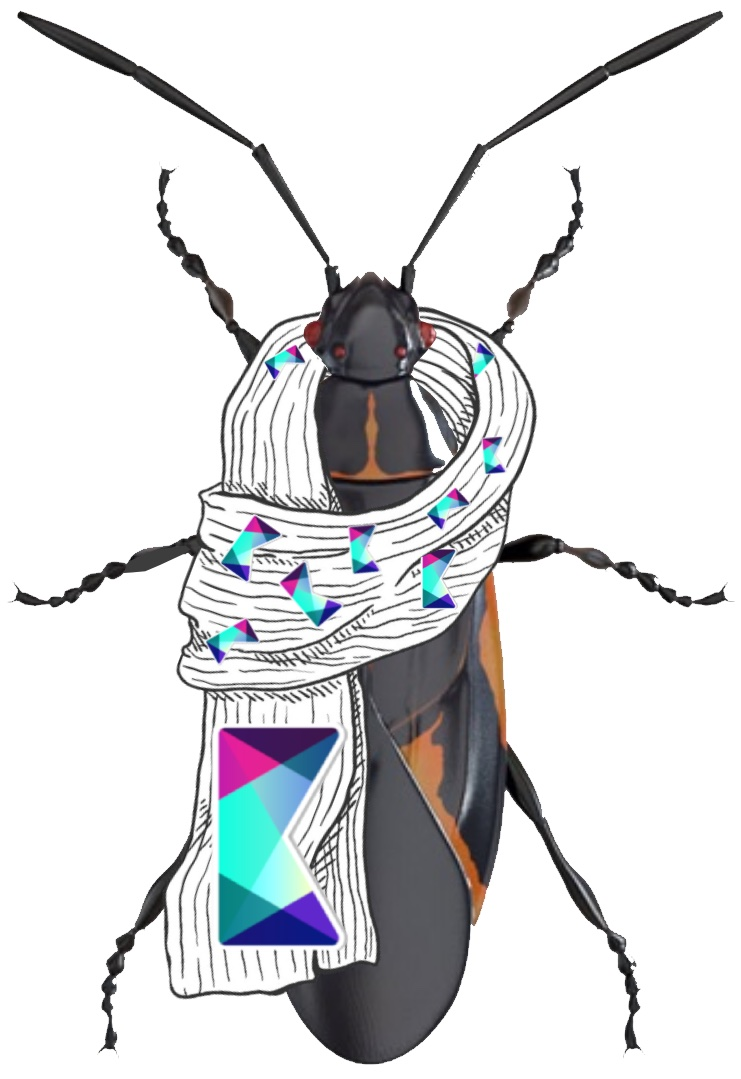
\includegraphics[height=5cm]{figures/kokkos-feature1} \end{center}
  {\tiny \textsuperscript{*}undocumented feature}
  \end{column}
\end{columns}
\end{frame}

\begin{frame}[fragile]{Contributing}
We welcome patches and other contributions to the project.

There are a few guidelines you need to follow.

\begin{itemize}
\item Make sure your pull request are against the \textbf{DEVELOP} branch
\item Follow our coding style (Apply \texttt{clang-format},\texttt{cmake-format})
\item Make sure tests pass (Configure with \texttt{-DKokkos\_ENABLE\_TESTS=ON}, build, run with \texttt{ctest})
\item Avoid mixing in unrelated changes
\item Describe the changes and provide a rational
\end{itemize}
\end{frame}

\begin{frame}[fragile]{Maintenance in progress}
\begin{center}
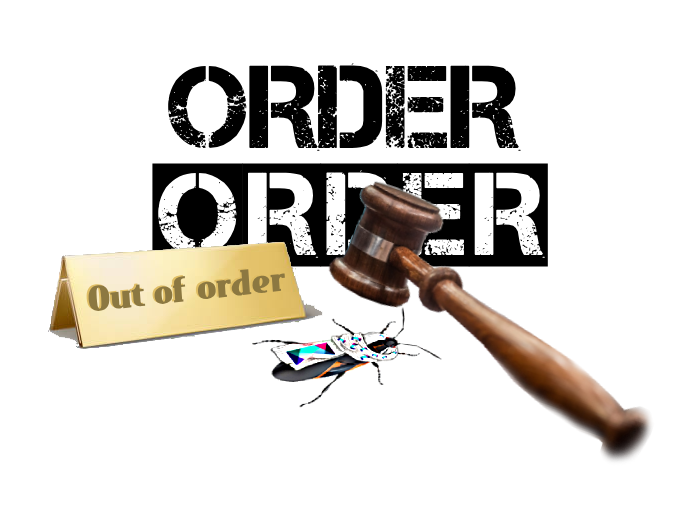
\includegraphics[width=0.65\textwidth]{figures/kokkos-orderorder}
\end{center}
\end{frame}

%%%%%%%%%%%%%%%%%%%%%%%%%%%%%%%%%%%%%%%%%%%%%%%%%%%%%%%%%%
\subsection{Roadmap}
\begin{frame}[fragile]{Release timeline}
\begin{center}
\textbf{We try to release on a 4 month cycle}
\vspace{1cm}

    \begin{tikzpicture}
\begin{axis}[
    width=\textwidth,
    date coordinates in=x,
    % date ZERO=2023-03-03,
    date ZERO=2020-01-31,
    % xmin=2023-01-03 00:00, xmax=2026-03-20 00:00,
    xmin=2019-11-03 00:00, xmax=2026-03-20 00:00,
    xtick={2019-11-03,2020-03-03,2020-07-03,2020-11-03,2021-03-03,2021-07-03,2021-11-03,2022-03-03,2022-07-03,2022-11-03,2023-03-03,2023-07-03,2023-11-03,2024-03-03,2024-07-03,2024-11-03,2025-03-03,2025-07-03,2025-11-03,2026-03-03},
    axis x line=bottom,% only show the bottom x axis
    xticklabel style={rotate=90,anchor=near xticklabel},
    xticklabel={\pgfcalendarmonthshortname{\month}/\year},
    hide y axis,
    ymin=0,ymax=6,
    y=0.2cm,
    scatter/classes={%
        a={mark=o,draw=black}}
    ]

\addplot[scatter,only marks,mark=x,
    mark size = 3pt,
    color = green]
coordinates {
  (2020-01-31 00:00, 1)
  (2020-04-14 00:00, 1)
  (2020-08-19 00:00, 1)
  (2020-12-16 00:00, 1)
  (2021-04-26 00:00, 1)
  (2021-11-19 00:00, 1)
  (2022-04-14 00:00, 1)
  (2022-08-25 00:00, 1)
    };
    \node [coordinate,pin=above:{3.0}]
        at (axis cs:2020-01-31,1)   {};
    \node [coordinate,pin=above:{3.7}]
        at (axis cs:2022-08-25,1) {};

\addplot[scatter,only marks,mark=x,
    mark size = 3pt,
    color = red]
coordinates {
  (2023-03-03 00:00, 1)
  (2023-06-28 00:00, 1)
  (2023-11-20 00:00, 1)
  (2024-04-04 00:00, 1)
  (2024-08-12 00:00, 1)
  (2024-11-25 00:00, 1)
  (2025-03-28 00:00, 1)
    };
    \node [coordinate,pin=above:{4.0}]
        at (axis cs:2023-03-03,1)   {};
    \node [coordinate,pin=above:{4.6}]
        at (axis cs:2025-03-28,1) {};

\addplot[scatter,only marks,mark=x,
    mark size = 3pt,
    color = black!40!white]
coordinates {
  (2025-07-20 00:00, 1)
  (2025-11-20 00:00, 1)
    };

    \node [coordinate,pin=above:{4.7}]
        at (axis cs:2025-07-20,1)   {};
    \node [coordinate,pin=above:{5.0}]
        at (axis cs:2025-11-20,1) {};

\end{axis}
\end{tikzpicture}
\end{center}

\end{frame}
  
\begin{frame}[fragile]{Kokkos 5 compiler requirements}

\textbf{New minimum compiler version requirements for C++20 support}

\begin{center}
\begin{tabular}{l|l}
  Clang(CPU)          & 14.0.0 \\ \hline
  Clang(CUDA)         & 14.0.0 \\ \hline
  Clang(OpenMPTarget) & 15.0.0 \\ \hline
  GCC                 & 10.1.0 \\ \hline
  Intel               & not supported \\ \hline
  IntelLLVM(CPU)      & 2022.0.0 \\ \hline
  IntelLLVM(SYCL)     & 2024.2.0 \\ \hline
  NVCC                & 12.0.0 \\ \hline
  HIPCC               & tbd \\ \hline
  NVHPC               & tbd \\ \hline
  MSVC                & 19.30
\end{tabular}
\vspace{-10pt}
\end{center}
\end{frame}

